\documentclass[12pt,a4paper]{article}

% ---------------------------------------------------------------
% Configuração geral - compatível com pdfLaTeX no Overleaf
% ---------------------------------------------------------------
\usepackage[T1]{fontenc}
\usepackage[utf8]{inputenc}
\usepackage[brazil]{babel}
\usepackage{times} % Fonte serifada Times, conforme artigo-modelo
\usepackage{microtype}
\usepackage{geometry}
\geometry{top=3cm,bottom=2cm,left=3cm,right=2cm}
\usepackage{setspace}
\setstretch{1.03} % Ajuste controlado para manter o relatório próximo de 20 páginas
\usepackage{ragged2e}
\justifying
\usepackage{graphicx}
\usepackage{booktabs}
\usepackage{array}
\usepackage{tabularx}
\usepackage{longtable}
\usepackage{multirow}
\usepackage[table]{xcolor}
\usepackage{enumitem}
\usepackage{tikz}
\usetikzlibrary{arrows.meta,positioning,shapes.geometric,fit,calc}
\usepackage{float}
\usepackage{caption}
\captionsetup{font=small,labelfont=bf,justification=centering}
\usepackage{url}
\usepackage[hidelinks]{hyperref} % URLs/citações sem coloração ou bordas
\usepackage[alf]{abntex2cite}
\usepackage{fancyhdr}
\usepackage{titlesec}

\usepackage{xcolor}
\newcommand\todoe[1]{\textcolor{red}{evandro:#1}}

% Paleta estritamente monocromática: texto preto, figuras em escala de cinza.
% Mantidos os nomes de cores anteriores para compatibilidade com as figuras TikZ.
\definecolor{LumeAzul}{gray}{0.15}
\definecolor{LumeMarinho}{gray}{0.0}
\definecolor{LumeVerde}{gray}{0.35}
\definecolor{LumeClaro}{gray}{0.95}
\definecolor{LumeMenta}{gray}{0.90}
\definecolor{LumeCinza}{gray}{0.96}

\titleformat{\section}{\normalfont\bfseries\Large}{\thesection}{0.6em}{}
\titleformat{\subsection}{\normalfont\bfseries\large}{\thesubsection}{0.6em}{}
\titleformat{\subsubsection}{\normalfont\bfseries\normalsize}{\thesubsubsection}{0.6em}{}
\setlength{\parindent}{1.25cm}
\setlength{\parskip}{0.10em}
\setlist[itemize]{leftmargin=1.1cm,itemsep=0.15em,topsep=0.25em}
\setcounter{secnumdepth}{3}
\setcounter{tocdepth}{2}
\renewcommand{\contentsname}{SUMÁRIO}
\renewcommand{\refname}{REFERÊNCIAS}

\pagestyle{fancy}
\fancyhf{}
\renewcommand{\headrulewidth}{0pt}
\renewcommand{\footrulewidth}{0.2pt}
\fancyfoot[L]{\footnotesize Agendinha -- Relatório de Projeto de Software}
\fancyfoot[R]{\footnotesize\thepage}

\newcommand{\autor}{Gabriella Marreto Rodrigues}
\newcommand{\titulo}{Desenvolvimento e avaliação de um PWA simples e de baixo custo para digitalização de agendamentos de microempreendedores}
\newcommand{\tituloingles}{Development and evaluation of a simple, low-cost PWA for digitizing appointments for microentrepreneurs}
\newcommand{\instituicao}{Universidade Tecnológica Federal do Paraná}
\newcommand{\curso}{Engenharia de Software}
\newcommand{\orientador}{Prof. Dr. Evandro Kuszera}
\newcommand{\cidade}{Dois Vizinhos}
\newcommand{\ano}{2026}

\newcolumntype{Y}{>{\raggedright\arraybackslash}X}
\newcommand{\fontepropria}{Fonte: autoria própria (2026).}

\begin{document}
\sloppy

% ---------------------------------------------------------------
% Capa
% ---------------------------------------------------------------
\begin{titlepage}
    \centering
    {\large\MakeUppercase{\instituicao}\par}
    {\large CURSO DE \MakeUppercase{\curso}\par}
    \vspace{3.2cm}
    {\large\MakeUppercase{\autor}\par}
    \vfill
    {\bfseries\Large\MakeUppercase{\titulo}\par}
    \vfill
    {\large\MakeUppercase{\cidade}\par}
    {\large\ano\par}
\end{titlepage}

% ---------------------------------------------------------------
% Folha de rosto
% ---------------------------------------------------------------
\begin{titlepage}
    \centering
    {\large\MakeUppercase{\autor}\par}
    \vspace{3cm}
    {\bfseries\Large\MakeUppercase{\titulo}\par}
    \vspace{0.5cm}
    {\itshape\tituloingles\par}
    \vspace{2.5cm}
    \begin{flushright}
        \begin{minipage}{0.52\textwidth}
        Trabalho de Conclusão de Curso de Graduação apresentado como requisito parcial para obtenção do título de Bacharel em Engenharia de Software pela Universidade Tecnológica Federal do Paraná (UTFPR).

        \vspace{0.5cm}
        \textbf{Orientador:} \orientador.
        \end{minipage}
    \end{flushright}
    \vfill
    {\large\MakeUppercase{\cidade}\par}
    {\large\ano\par}
\end{titlepage}

% ---------------------------------------------------------------
% Folha de aprovação - preencher antes da entrega
% ---------------------------------------------------------------
\begin{titlepage}
    \centering
    {\large\MakeUppercase{\autor}\par}
    \vspace{1.5cm}
    {\bfseries\large\MakeUppercase{\titulo}\par}
    \vspace{1cm}
    Trabalho de Conclusão de Curso de Graduação apresentado como requisito parcial para obtenção do título de Bacharel em Engenharia de Software.

    \vspace{0.8cm}
    Aprovado em: \underline{\hspace{1cm}} de \underline{\hspace{3cm}} de 2026.

    \vspace{1cm}
    \textbf{BANCA EXAMINADORA}

    \vspace{1.2cm}
    \rule{10cm}{0.4pt}\\
    \orientador{} -- Orientador\\
    Universidade Tecnológica Federal do Paraná

    \vspace{1.2cm}
    \rule{10cm}{0.4pt}\\
    Prof.(a) Dr.(a) \underline{\hspace{5cm}}\\
    Universidade Tecnológica Federal do Paraná

    \vspace{1.2cm}
    \rule{10cm}{0.4pt}\\
    Prof.(a) Dr.(a) \underline{\hspace{5cm}}\\
    Universidade Tecnológica Federal do Paraná
\end{titlepage}

\pagenumbering{roman}
\setcounter{page}{4}

\tableofcontents
\newpage

\pagenumbering{arabic}
\setcounter{page}{1}

\section{INTRODUÇÃO}

\subsection{Contextualização e justificativa}

O acesso a ferramentas digitais de agendamento não deve depender da capacidade de contratar sistemas complexos ou de manter uma despesa mensal elevada. A Agendinha foi concebida para profissionais autônomos e microempreendedores de renda limitada que atendem com horário marcado, como barbeiros, manicures e prestadores de cuidados pessoais. A proposta consiste em oferecer uma forma direta de disponibilizar a agenda e receber reservas pela internet, sem exigir que o cliente instale aplicativos ou crie uma conta. O valor pretendido é tornar a digitalização viável inclusive para quem administra o negócio sozinho e dispõe de pouco tempo e recursos financeiros.

A gestão de agendamentos representa um desafio operacional para profissionais autônomos e pequenos prestadores de serviços, especialmente quando realizada por meio de registros manuais ou aplicativos de mensagens. Nesse contexto, a definição de horários depende de interações sucessivas entre clientes e prestadores, exigindo consultas frequentes à disponibilidade e atualizações individuais da agenda. Esse processo pode aumentar o esforço administrativo, dificultar a organização dos compromissos e gerar atrasos na confirmação dos atendimentos. Diante desse cenário, identifica-se a oportunidade de desenvolver uma solução digital acessível que centralize a disponibilidade de horários e permita aos próprios clientes realizar seus agendamentos de forma autônoma, reduzindo a necessidade de intermediação manual e simplificando a rotina dos profissionais.

A aplicação procura eliminar a negociação repetitiva sem eliminar a proximidade do atendimento. O prestador cadastra os períodos em que pode trabalhar e compartilha um endereço web, inclusive por aplicativos de mensagens que já utiliza. Ao acessar esse link, o cliente visualiza os horários disponíveis, escolhe por conta própria a opção conveniente e efetua a reserva sem cadastro prévio e sem download. O propósito de experiência é que essa interação seja tão simples quanto conversar pelo celular, idealmente com menos etapas.

A dimensão social e econômica dessa escolha encontra respaldo na relevância do microempreendedorismo de serviços. O IBGE contabilizou 14,6 milhões de microempreendedores individuais (MEIs) no Brasil em 2022; 51,5\% atuavam em serviços e cerca de 1,3 milhão exerciam atividades de cabeleireiro e outros tratamentos de beleza \cite{ibgemei}. O mesmo levantamento identificou aproximadamente 4,1 milhões de MEIs inscritos no Cadastro Único (28,4\% do total), evidenciando a presença de uma parcela economicamente vulnerável entre os empreendedores formalizados \cite{ibgemei}. A inscrição no Cadastro Único não caracteriza automaticamente a renda de cada potencial usuário da Agendinha, mas sustenta a importância de analisar soluções cujos custos fixos não comprometam a sustentabilidade de negócios pequenos.

O mercado já possui plataformas de agendamento. Muitas delas integradas a ferramentas administrativas mais amplas. O Booksy anuncia assinatura de R\$ 99,99 mensais, acrescida de impostos, com recursos de marketing, pagamento e relatórios \cite{booksypricing}. A Trinks divulga mensalidade de R\$ 110 no ciclo mensal para estabelecimentos com um ou dois profissionais \cite{trinkspricing}. O Reservio disponibiliza plano gratuito com limite de até 40 agendamentos a cada 30 dias e oferece planos pagos com capacidades superiores \cite{reserviopricing}. Tais serviços atendem necessidades legítimas, mas permitem evidenciar a diferença de escopo pretendida: a Agendinha não busca reproduzir um sistema completo de administração comercial, e sim disponibilizar o núcleo essencial da agenda digital com a menor barreira possível de acesso.

Dessa forma, a proposta de valor articula três compromissos: \textbf{simplicidade para o cliente}, que não precisa criar conta nem instalar aplicativo; \textbf{autonomia para o prestador}, que publica os horários disponíveis e reduz a necessidade de negociações manuais; e \textbf{acessibilidade econômica}, por meio de infraestrutura gerenciada e compartilhada, com preocupação explícita com o custo mensal por profissional. O estudo de viabilidade apresentado adiante estima cenários de infraestrutura, mas não comprova ainda uma mensalidade final, uma economia efetiva de tempo ou uma superioridade de usabilidade. Esses aspectos dependerão de dados operacionais e da avaliação com o público-alvo. A Tabela~\ref{tab:comparacao} compara características e preços anunciados pelas soluções consultadas em 25 de outubro de 2026.

\begin{figure}[H]
    \centering
    \resizebox{0.95\textwidth}{!}{\begin{tikzpicture}[
    font=\small,
    node distance=5mm,
    blocoManual/.style={draw=black!45,fill=black!6,rounded corners,minimum width=5.3cm,minimum height=1.15cm,align=center},
    blocoDigital/.style={draw=LumeVerde!70,fill=LumeMenta,rounded corners,minimum width=5.3cm,minimum height=1.15cm,align=center},
    setaManual/.style={-{Stealth[length=2mm]},black!75,thick},
    setaDigital/.style={-{Stealth[length=2mm]},LumeVerde,thick}
]
\node[font=\bfseries] (hm) at (0,0) {PROCESSO MANUAL};
\node[font=\bfseries] (hd) at (7,0) {PROCESSO DIGITAL PROPOSTO};

\node[blocoManual,below=5mm of hm] (m1) {\textbf{Pedido em mensagem}\\cliente pergunta horários};
\node[blocoManual,below=of m1] (m2) {\textbf{Consulta ao caderno}\\prestador verifica manualmente};
\node[blocoManual,below=of m2] (m3) {\textbf{Anotação}\\risco de conflito ou perda};
\node[blocoManual,below=of m3] (m4) {\textbf{Confirmação manual}\\nova troca de mensagens};

\node[blocoDigital,below=5mm of hd] (d1) {\textbf{Link público}\\sem cadastro do cliente};
\node[blocoDigital,below=of d1] (d2) {\textbf{Horários disponíveis}\\cálculo automático};
\node[blocoDigital,below=of d2] (d3) {\textbf{Reserva transacional}\\sem sobreposição};
\node[blocoDigital,below=of d3] (d4) {\textbf{Confirmação automática}\\e-mail e histórico};

\draw[setaManual] (m1) -- (m2);
\draw[setaManual] (m2) -- (m3);
\draw[setaManual] (m3) -- (m4);
\draw[setaDigital] (d1) -- (d2);
\draw[setaDigital] (d2) -- (d3);
\draw[setaDigital] (d3) -- (d4);
\draw[dashed,gray!60] (3.5,-0.3) -- (3.5,-7.1);
\end{tikzpicture}
}
    \caption{Comparação entre o processo manual e o fluxo digital proposto.}
    \label{fig:processo}
    \fontepropria
\end{figure}

\subsection{Problema}

\begin{quote}
\textit{Como permitir que prestadores de serviços de renda limitada digitalizem seus agendamentos com baixo custo mensal e uma experiência tão simples quanto a troca habitual de mensagens, sem exigir cadastro ou instalação por parte do cliente?}
\end{quote}

A questão orienta o produto e os critérios de avaliação. A solução deve permitir que o cliente escolha autonomamente entre horários disponíveis, enquanto o prestador evita consultas e respostas repetitivas. A simplicidade percebida e a economia real deverão ser verificadas com usuários e dados de operação.

\subsection{Objetivos}

\subsubsection{Objetivo geral}

Desenvolver uma aplicação web de agendamentos simples e economicamente acessível para prestadores de serviços de baixa renda, permitindo que clientes consultem a disponibilidade e reservem horários sem cadastro ou instalação, com avaliação de sua adequação ao público-alvo em etapa posterior.

\subsubsection{Objetivos específicos}

\begin{itemize}
    \item permitir que o prestador configure seus horários de atendimento com poucos passos e compartilhe um endereço público;
    \item oferecer ao cliente visualização intuitiva da disponibilidade e reserva sem criação de conta ou instalação de aplicativo;
    \item impedir sobreposição de reservas confirmadas, inclusive diante de solicitações concorrentes;
    \item automatizar confirmações, cancelamentos e avisos sem prolongar a resposta da operação principal;
    \item oferecer instalação como PWA e priorizar a experiência em telas móveis;
    \item estimar e buscar reduzir o custo mensal por prestador com infraestrutura gerenciada e compartilhada, preservando a acessibilidade econômica;
    \item documentar critérios para avaliação futura da facilidade de uso com pessoas do público-alvo, sem presumir resultados ainda não coletados.
\end{itemize}

\subsection{Descrição das regras de negócio e escopo}

O escopo foi conferido contra o esquema SQL e os contratos atuais do backend. A descrição a seguir considera o comportamento implementado na versão documentada.

\begin{table}[H]
\centering
\caption{Regras de negócio centrais.}
\label{tab:regras}
\small
\begin{tabularx}{\textwidth}{p{3.2cm}Y}
\toprule
\textbf{Regra} & \textbf{Comportamento implementado} \\
\midrule
Identidade pública & Cada prestador possui perfil, fuso horário e slug único que compõe seu link. \\
Disponibilidade & Grupos ativos definem regras semanais; exceções acrescentam ou bloqueiam intervalos; reservas e horários passados são removidos do resultado. \\
Reserva & O cliente informa nome, e-mail e telefone sem criar conta. A gravação usa transação, idempotência e restrição contra sobreposição. \\
Cancelamento & O prestador autenticado ou o cliente portador de token válido pode cancelar. O registro passa a \texttt{CANCELLED} e permanece no histórico. \\
Cache & Alterações relevantes avançam a versão da agenda. O Redis guarda apenas resultados temporários e sua falha leva à consulta ao PostgreSQL. \\
Comunicação & E-mails e avisos são persistidos em outboxes e processados por workers, permitindo repetição controlada. \\
\bottomrule
\end{tabularx}
\fontepropria
\end{table}

Ficam fora do produto mínimo: pagamentos, gestão financeira, estoque, marketplace, duração variável por serviço, relatórios analíticos e reagendamento. Essa contenção é deliberada: a proposta não é reproduzir uma suíte administrativa, mas digitalizar o núcleo da agenda em papel.


\section{DESENVOLVIMENTO}

\subsection{Especificação das funcionalidades}

As funcionalidades foram organizadas por ator e verificadas na interface, nos hooks, nos contratos das Edge Functions e nas migrações do banco de dados. A classificação distingue o que possui fluxo de uso completo do que existe apenas como suporte técnico.

\begin{table}[htbp]
\centering
\caption{Funcionalidades e situação da implementação.}
\label{tab:funcionalidades}
\scriptsize
\begin{tabularx}{\textwidth}{>{\RaggedRight\arraybackslash}p{1.7cm}Y>{\RaggedRight\arraybackslash}p{4.0cm}}
\toprule
\textbf{Ator} & \textbf{Funcionalidade} & \textbf{Situação} \\
\midrule
Prestador & Cadastro e login por e-mail ou Google & Implementada \\
Prestador & Perfil, slug público e fuso horário & Implementada \\
Prestador & Grupos de horários, dias e faixas de atendimento & Implementada \\
Prestador & Agenda diária e estados dos compromissos & Implementada \\
Prestador & Bloqueio, horário extra, liberação e cancelamento & Implementada \\
Prestador & Avisos, Web Push e instalação como PWA & Implementada; entrega requer configuração e worker operacional \\
Prestador & Listagem de clientes & Parcial: API e hook existem; não há tela dedicada \\
Cliente & Acesso por link, seleção de data e horário & Implementada \\
Cliente & Reserva com nome, e-mail e telefone, sem conta & Implementada \\
Cliente & Confirmação por e-mail e cancelamento por token & Implementada; envio requer worker operacional \\
\bottomrule
\end{tabularx}
\fontepropria
\end{table}

\subsubsection{Fluxo do prestador}

Após autenticar-se, o prestador configura nome público, endereço curto e fuso horário. Em seguida, cria um grupo de disponibilidade, seleciona dias da semana e informa o início, a duração e a quantidade de atendimentos de cada faixa. A agenda diária reúne horários livres, bloqueios e reservas. Um intervalo específico pode ser bloqueado ou liberado sem alterar toda a recorrência; uma reserva pode ser cancelada, mas não apagada.

\subsubsection{Fluxo do cliente}

O cliente abre o link do prestador, escolhe uma data e um dos horários calculados pelo backend, preenche seus dados de contato e confirma. A API volta a validar a disponibilidade durante a transação, evitando que a seleção feita na tela seja tratada como garantia de reserva. O e-mail resultante contém o resumo e um link de cancelamento associado a token próprio.

\subsubsection{Registro visual da aplicação}

O fluxo de uso é representado por duas telas principais: a configuração de disponibilidade pelo prestador e a seleção de horários na página pública de reserva. Essas interfaces ilustram as funcionalidades centrais da Agendinha.

\begin{figure}[htbp]
    \centering

    \begin{minipage}[t]{0.47\textwidth}
        \centering
        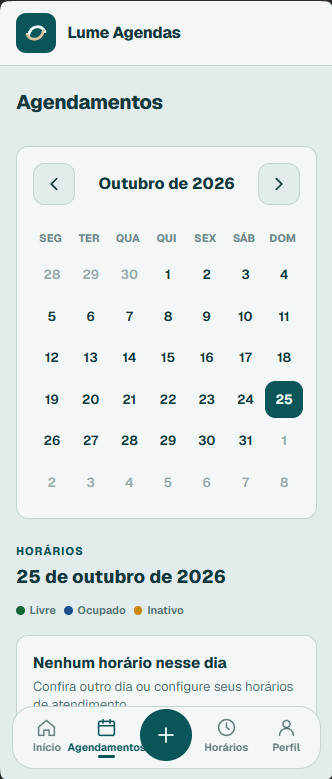
\includegraphics[
            width=\linewidth,
            height=6cm,
            keepaspectratio
        ]{agendinha-prestador.png}

        \caption{Configuração de horários do prestador.}
        \label{fig:tela-prestador}
    \end{minipage}
    \hfill
    \begin{minipage}[t]{0.47\textwidth}
        \centering
        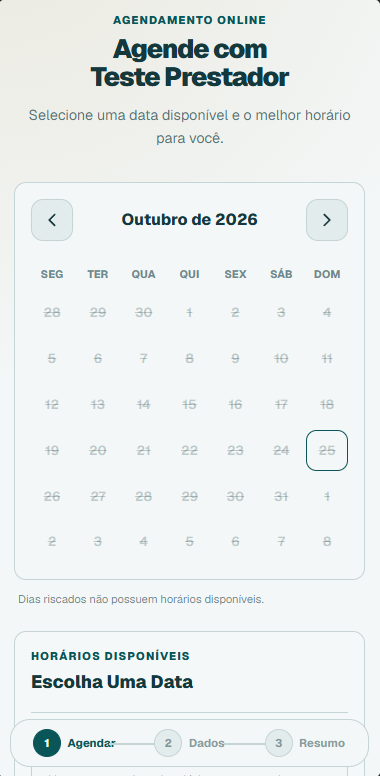
\includegraphics[
            width=\linewidth,
            height=6cm,
            keepaspectratio
        ]{agendinha-cliente.png}

        \caption{Seleção de horários pelo cliente.}
        \label{fig:tela-cliente}
    \end{minipage}
\end{figure}

Uma demonstração contínua dos fluxos da aplicação está disponível no \href{https://drive.google.com/drive/folders/1Iy3Y8jWdIG8WkwKIMk8nMqgSO8XAoJEi?usp=sharing}{vídeo de demonstração da Agendinha}.

\subsubsection{Critério de simplicidade}

Simplicidade não é medida apenas pelo número de telas. O desenho reduz decisões: o cliente não escolhe plano, não instala aplicativo e não cria senha; o prestador não precisa configurar infraestrutura. A avaliação exploratória proposta na Seção~\ref{sec:avaliacao} verificará se essa redução se converte em tarefas concluídas e quais dificuldades permanecem.

\FloatBarrier

\subsection{Arquitetura e fluxos do sistema}

A aplicação foi organizada em cliente web, serviços de backend, persistência e provedores especializados. A Figura~\ref{fig:arquitetura} apresenta os atores, componentes e serviços efetivamente utilizados pela Agendinha. As regras de domínio não dependem do estado local da tela: passam pelas Edge Functions, que coordenam autenticação, dados, cache e comunicação.

\begin{figure}[htbp]
    \centering
    \resizebox{\textwidth}{!}{\begin{tikzpicture}[
    font=\scriptsize,
    caixa/.style={draw=LumeAzul,fill=LumeClaro,rounded corners,minimum width=2.55cm,minimum height=1.35cm,align=center},
    servico/.style={draw=LumeVerde,fill=LumeMenta,rounded corners,minimum width=2.75cm,minimum height=1.35cm,align=center},
    dado/.style={draw=black!65!black,fill=black!8,rounded corners,minimum width=2.75cm,minimum height=1.35cm,align=center},
    seta/.style={-{Stealth[length=2mm]},LumeAzul,thick}
]
\node[caixa] (prestador) at (0,2.2) {\textbf{Prestador}\\painel autenticado};
\node[servico] (cliente) at (0,-0.2) {\textbf{Cliente}\\link público};
\node[caixa] (pwa) at (4,1) {\textbf{Next.js / PWA}\\React + TypeScript\\service worker};
\node[caixa] (auth) at (8,3) {\textbf{Supabase Auth}\\login + JWT};
\node[servico] (edge) at (8,1) {\textbf{Edge Functions}\\regras de negócio};
\node[dado] (postgres) at (8,-1) {\textbf{PostgreSQL}\\fonte oficial + RLS};
\node[caixa] (blackis) at (12,3) {\textbf{Upstash Redis}\\cache temporário};
\node[servico] (resend) at (12,1) {\textbf{Resend}\\e-mail};
\node[dado] (push) at (12,-1) {\textbf{Web Push}\\avisos};

\draw[seta] (prestador) -- (pwa);
\draw[seta] (cliente) -- (pwa);
\draw[seta] (pwa) -- node[above,sloped]{autentica} (auth);
\draw[seta] (pwa) -- node[above]{HTTPS} (edge);
\draw[seta] (edge) -- node[right]{SQL} (postgres);
\draw[seta] (edge) -- node[above,sloped]{cache} (blackis);
\draw[seta] (edge) -- node[above]{outbox} (resend);
\draw[seta] (edge) -- node[above,sloped]{avisos} (push);

\node[align=center,font=\scriptsize] at (6,-2.25) {Páginas: Network-First; recursos estáticos: cache local.\\Falha do Redis: consulta direta ao PostgreSQL.};
\end{tikzpicture}
}
    \caption{Arquitetura implementada da Agendinha.}
    \label{fig:arquitetura}
    \fontepropria
\end{figure}

\subsubsection{Atores, frontend e PWA}

A caixa \textbf{Prestador} representa o usuário autenticado que administra perfil, disponibilidade, exceções e compromissos. A caixa \textbf{Cliente} representa quem acessa o link público, consulta horários, reserva e cancela sem possuir conta. Ambos utilizam a mesma aplicação \textbf{Next.js/PWA}, construída com React e TypeScript, mas seguem rotas, permissões e contratos distintos.

O manifesto permite instalar a aplicação, e o service worker aplica Network-First às navegações para priorizar conteúdo atualizado e oferecer uma página de contingência quando não há conexão. Recursos estáticos elegíveis usam cache local; rotas de autenticação não são armazenadas. A interface pode registrar a inscrição do navegador para receber notificações Web Push quando o prestador concede permissão.

\subsubsection{Autenticação e regras de negócio}

O \textbf{Supabase Auth} mantém a identidade do prestador, oferece cadastro por e-mail e autenticação com Google e emite o JWT usado nas operações privadas. A interface não recebe credenciais administrativas. As \textbf{Edge Functions} validam entradas e origem, identificam o prestador, aplicam limites às rotas públicas e executam os casos de uso por meio de consultas e funções transacionais do banco.

Operações privadas combinam a validação do JWT com políticas de Row Level Security. Operações públicas, como consulta de disponibilidade e reserva, recebem validação específica e não expõem acesso irrestrito às tabelas. Esse desenho mantém a autorização no servidor, mesmo quando a interface antecipa validações para melhorar a experiência de preenchimento.

\subsubsection{Dados, cache e comunicações}

O \textbf{PostgreSQL} é a fonte oficial do estado de perfis, regras, clientes e reservas. Chaves estrangeiras, verificações, transações, RLS e a restrição de exclusão de intervalos protegem a consistência. O \textbf{Upstash Redis} mantém apenas disponibilidade derivada e controles auxiliares. As chaves incorporam o prestador, a data, a versão do esquema de cache e a versão da agenda; o TTL é configurável entre 10 e 900 segundos, com padrão de 60 segundos. Falhas de leitura ou gravação no Redis não interrompem a consulta ao banco.

O \textbf{Resend} transporta e-mails de confirmação e cancelamento. O \textbf{Web Push} entrega avisos de novas reservas e cancelamentos aos navegadores inscritos. Nenhum desses provedores participa da transação principal: eventos são gravados nas tabelas de outbox e consumidos por workers. Tentativas, falhas e reagendamentos permanecem registrados, de forma que uma indisponibilidade de comunicação não invalida uma reserva já confirmada.

\subsubsection{Fluxos críticos e tratamento de falhas}

A Figura~\ref{fig:fluxos} reúne a consulta de disponibilidade e a criação da reserva. Os fluxos conectam as caixas da arquitetura e mostram por que o cache acelera leituras, mas não substitui a validação transacional no PostgreSQL.

\begin{figure}[htbp]
    \centering
    \resizebox{\textwidth}{!}{\begin{tikzpicture}[
    font=\scriptsize,
    ator/.style={draw=LumeAzul!35,fill=LumeClaro,rounded corners,minimum width=1.6cm,minimum height=0.65cm,align=center},
    vida/.style={gray!55,dashed},
    msg/.style={-{Stealth[length=1.8mm]},LumeAzul,thick},
    msgb/.style={-{Stealth[length=1.8mm]},LumeVerde,thick}
]
\node[font=\bfseries] at (2.8,0.5) {A. CONSULTA DE DISPONIBILIDADE};
\node[ator] (c1) at (0,0) {Cliente};
\node[ator] (e1) at (2,0) {Edge};
\node[ator] (r1) at (4,0) {Redis};
\node[ator] (p1) at (6,0) {Postgres};
\foreach \x in {0,2,4,6}{\draw[vida] (\x,-0.35) -- (\x,-5.7);}
\draw[msg] (0,-0.8) -- node[above]{GET slots} (2,-0.8);
\draw[msg] (2,-1.5) -- node[above]{GET chave} (4,-1.5);
\draw[msg] (4,-2.2) -- node[above]{hit: dados} (2,-2.2);
\draw[msg] (2,-3.0) -- node[above]{miss: consulta} (6,-3.0);
\draw[msg] (6,-3.7) -- node[above]{dados oficiais} (2,-3.7);
\draw[msg] (2,-4.4) -- node[above]{SET + TTL} (4,-4.4);
\draw[msg] (2,-5.1) -- node[above]{horários} (0,-5.1);

\draw[gray!50] (7,-0.4) -- (7,-5.7);
\node[font=\bfseries] at (10.6,0.5) {B. RESERVA E CONFIRMAÇÃO};
\node[ator] (c2) at (8,0) {Cliente};
\node[ator] (e2) at (10,0) {Edge};
\node[ator] (p2) at (12,0) {Postgres};
\node[ator] (w2) at (14,0) {Workers};
\foreach \x in {8,10,12,14}{\draw[vida] (\x,-0.35) -- (\x,-5.7);}
\draw[msgb] (8,-0.8) -- node[above]{POST + chave} (10,-0.8);
\draw[msgb] (10,-1.6) -- node[above]{RPC transacional} (12,-1.6);
\node[draw=LumeVerde,minimum width=0.45cm,minimum height=0.45cm] at (12.25,-2.35) {};
\node[right] at (12.55,-2.35) {valida e bloqueia};
\node[draw=LumeVerde,minimum width=0.45cm,minimum height=0.45cm] at (12.25,-3.0) {};
\node[right] at (12.55,-3.0) {agenda + outbox};
\draw[msgb] (12,-3.7) -- node[above]{commit} (10,-3.7);
\draw[msgb] (10,-4.4) -- node[above]{confirmação} (8,-4.4);
\draw[msgb] (14,-5.1) -- node[above]{consome outbox} (12,-5.1);
\end{tikzpicture}
}
    \caption{Consulta de disponibilidade e criação de reserva.}
    \label{fig:fluxos}
    \fontepropria
\end{figure}

Na consulta, o cliente solicita um dia ou período pelo frontend. A Edge Function identifica o perfil pelo slug e busca no Redis as chaves correspondentes à versão corrente da agenda. Em um acerto, os horários validados são devolvidos sem nova leitura do PostgreSQL. Em uma ausência ou falha do Redis, o backend calcula os intervalos com base nos grupos ativos, regras semanais, exceções, reservas confirmadas e fuso horário. O resultado é devolvido mesmo sem cache e, quando possível, armazenado com TTL para consultas seguintes.

Na reserva, a Edge Function valida slug, intervalo, nome, e-mail, telefone e chave de idempotência. A função transacional volta a conferir se o período pertence à disponibilidade, normaliza os dados do cliente, mantém o vínculo com o prestador e tenta inserir o agendamento. A restrição de exclusão no PostgreSQL decide conflitos concorrentes: somente uma das solicitações pode manter o mesmo intervalo confirmado. A resposta da operação é vinculada à chave de idempotência para impedir duplicidade em reenvios.

Na mesma transação são criados o agendamento e os eventos necessários às outboxes. Depois do commit, a versão da agenda no Redis é incrementada, tornando obsoletas as chaves anteriores sem depender de sua remoção imediata. A resposta de sucesso retorna ao cliente antes do envio das mensagens. Workers separados reivindicam registros pendentes, chamam Resend e Web Push e registram sucesso, falha ou nova tentativa. Assim, erros no cache ou nos provedores de comunicação degradam recursos auxiliares, mas não alteram a decisão de integridade tomada pelo banco.

\FloatBarrier

\subsection{Persistência e integridade dos dados}

A persistência separa disponibilidade recorrente, exceções, identidade dos clientes, reservas e suporte operacional. O esquema é definido por migrações SQL e utiliza tipos nativos do PostgreSQL, chaves estrangeiras, unicidade, verificações de intervalo e políticas de acesso. A Figura~\ref{fig:der} apresenta as onze tabelas persistentes na versão documentada, com tipos, chaves e cardinalidades.

O perfil estende a identidade administrada pelo Supabase Auth. Cada perfil possui grupos de horários, e cada grupo reúne regras por dia da semana. A duração do atendimento e a quantidade de horários são armazenadas na regra, enquanto exceções representam bloqueios ou disponibilidade adicional. A separação entre \texttt{Client} e \texttt{ProviderClient} permite reutilizar a identidade do cliente e preservar os dados informados no relacionamento com cada prestador.

\begin{landscape}
\thispagestyle{fancy}
\vspace*{-0.6cm}
\noindent\begin{minipage}[t]{\linewidth}
\captionsetup{hypcap=false}
\captionof{figure}{Diagrama entidade-relacionamento da Agendinha.}
\label{fig:der}
\centering
\resizebox{0.90\linewidth}{!}{\begin{tikzpicture}[
    font=\scriptsize,
    entidade/.style={draw=black!80,fill=white,inner sep=2pt,align=left,anchor=north west},
    rel/.style={-{Stealth[length=1.5mm]},black!70,thin},
    rotulo/.style={fill=white,inner sep=1pt,font=\scriptsize}
]

\node[entidade] (profiles) at (0,0) {
\begin{tabular}{@{}lll@{}}
\rowcolor{black!15}\multicolumn{3}{c}{\textbf{profiles}}\\
PK/FK & \texttt{id} & uuid\\
 & \texttt{name} & text\\
UQ & \texttt{public\_slug} & text\\
 & \texttt{phone} & text?\\
 & \texttt{timezone} & text\\
 & \texttt{updated\_at} & timestamptz
\end{tabular}};

\node[entidade] (groups) at (6.4,0) {
\begin{tabular}{@{}lll@{}}
\rowcolor{black!15}\multicolumn{3}{c}{\textbf{AvailabilityRuleGroup}}\\
PK & \texttt{id} & uuid\\
FK & \texttt{provider\_id} & uuid\\
 & \texttt{name} & text\\
 & \texttt{is\_active} & boolean
\end{tabular}};

\node[entidade] (rules) at (13,0) {
\begin{tabular}{@{}lll@{}}
\rowcolor{black!15}\multicolumn{3}{c}{\textbf{AvailabilityRule}}\\
PK & \texttt{id} & uuid\\
FK & \texttt{group\_id} & uuid\\
 & \texttt{day\_of\_week} & smallint\\
 & \texttt{start\_time} & time\\
 & \texttt{end\_time} & time\\
 & \texttt{slot\_duration\_minutes} & smallint\\
 & \texttt{appointment\_count} & smallint
\end{tabular}};

\node[entidade] (idempotency) at (20.4,0) {
\begin{tabular}{@{}lll@{}}
\rowcolor{black!15}\multicolumn{3}{c}{\textbf{idempotency\_record}}\\
PK & \texttt{operation} & text\\
PK & \texttt{idempotency\_key} & uuid\\
 & \texttt{request\_hash} & text\\
 & \texttt{response} & jsonb\\
 & \texttt{created\_at} & timestamptz
\end{tabular}};

\node[entidade] (overrides) at (0,-4.8) {
\begin{tabular}{@{}lll@{}}
\rowcolor{black!15}\multicolumn{3}{c}{\textbf{AvailabilityOverride}}\\
PK & \texttt{id} & uuid\\
FK & \texttt{provider\_id} & uuid\\
 & \texttt{start\_datetime} & timestamptz\\
 & \texttt{end\_datetime} & timestamptz\\
 & \texttt{is\_available} & boolean
\end{tabular}};

\node[entidade] (clients) at (6.4,-4.8) {
\begin{tabular}{@{}lll@{}}
\rowcolor{black!15}\multicolumn{3}{c}{\textbf{Client}}\\
PK & \texttt{id} & uuid\\
 & \texttt{name} & text\\
UQ & \texttt{email} & text\\
 & \texttt{phone} & text
\end{tabular}};

\node[entidade] (providerclients) at (12.3,-4.8) {
\begin{tabular}{@{}lll@{}}
\rowcolor{black!15}\multicolumn{3}{c}{\textbf{ProviderClient}}\\
PK & \texttt{id} & uuid\\
FK & \texttt{provider\_id} & uuid\\
FK & \texttt{client\_id} & uuid\\
 & \texttt{name} & text\\
UQ & \texttt{email} & text\\
 & \texttt{phone} & text
\end{tabular}};

\node[entidade] (appointments) at (19.5,-4.8) {
\begin{tabular}{@{}lll@{}}
\rowcolor{black!15}\multicolumn{3}{c}{\textbf{Appointment}}\\
PK & \texttt{id} & uuid\\
FK & \texttt{provider\_id} & uuid\\
FK & \texttt{client\_id} & uuid\\
 & \texttt{start\_datetime} & timestamptz\\
 & \texttt{end\_datetime} & timestamptz\\
 & \texttt{status} & appointment\_status\\
UQ & \texttt{cancellation\_token} & uuid
\end{tabular}};

\node[entidade] (push) at (0,-9.8) {
\begin{tabular}{@{}lll@{}}
\rowcolor{black!15}\multicolumn{3}{c}{\textbf{push\_subscription}}\\
PK & \texttt{id} & uuid\\
FK & \texttt{provider\_id} & uuid\\
 & \texttt{endpoint} & text\\
 & \texttt{p256dh} & text\\
 & \texttt{auth\_key} & text\\
 & \texttt{created\_at} & timestamptz
\end{tabular}};

\node[entidade] (notices) at (8,-9.8) {
\begin{tabular}{@{}lll@{}}
\rowcolor{black!15}\multicolumn{3}{c}{\textbf{notice\_outbox}}\\
PK & \texttt{id} & uuid\\
FK & \texttt{provider\_id} & uuid\\
 & \texttt{event\_type} & notice\_event\_type\\
FK & \texttt{appointment\_id} & uuid\\
 & \texttt{status} & notice\_status\\
 & \texttt{push\_status} & notice\_push\_status\\
 & \texttt{push\_attempt\_count} & integer\\
 & \texttt{push\_available\_at} & timestamptz\\
 & \texttt{push\_locked\_at} & timestamptz?\\
 & \texttt{created\_at} & timestamptz\\
 & \texttt{dismissed\_at} & timestamptz?
\end{tabular}};

\node[entidade] (emails) at (19,-9.8) {
\begin{tabular}{@{}lll@{}}
\rowcolor{black!15}\multicolumn{3}{c}{\textbf{email\_outbox}}\\
PK & \texttt{id} & uuid\\
 & \texttt{event\_type} & email\_event\_type\\
FK & \texttt{appointment\_id} & uuid\\
 & \texttt{status} & email\_outbox\_status\\
 & \texttt{attempt\_count} & integer\\
 & \texttt{available\_at} & timestamptz\\
 & \texttt{locked\_at} & timestamptz?\\
 & \texttt{sent\_at} & timestamptz?\\
 & \texttt{last\_error} & text?\\
 & \texttt{created\_at} & timestamptz
\end{tabular}};

\draw[rel] (profiles.east) -- node[rotulo,above]{1:N} (groups.west);
\draw[rel] (groups.east) -- node[rotulo,above]{1:N} (rules.west);
\draw[rel] (profiles.south) -- node[rotulo,right]{1:N} (overrides.north);
\draw[rel] (clients.east) -- node[rotulo,above]{1:N} (providerclients.west);
\draw[rel] (providerclients.east) -- node[rotulo,above]{1:N, FK composta} (appointments.west);
\draw[rel] (profiles.south east) to[out=-25,in=150] node[rotulo,above]{1:N} (providerclients.north west);
\draw[rel] (clients.north east) to[out=30,in=150] node[rotulo,above]{1:N} (appointments.north west);
\draw[rel] (profiles.north) -- ++(0,1.1) -| node[rotulo,near end,right]{1:N} (appointments.east);
\draw[rel] (profiles.west) -- ++(-0.8,0) |- node[rotulo,near end,left]{1:N} (push.west);
\draw[rel] (appointments.south) to[out=-80,in=70] node[rotulo,right]{1:N} (emails.north);
\draw[rel] (appointments.south west) to[out=-115,in=40] node[rotulo,above]{1:N} (notices.north east);
\draw[rel] (profiles.west) -- ++(-1.15,0) |- (0,-15.5) -- node[rotulo,near end,below]{1:N} (notices.south);

\node[anchor=west,font=\scriptsize] at (0,-16.2) {Legenda: PK = chave primária; FK = chave estrangeira; UQ = restrição de unicidade; ``?'' = campo opcional.};
\node[anchor=east,font=\scriptsize] at (27,-16.2) {\texttt{profiles.id} também referencia \texttt{auth.users.id}.};

\end{tikzpicture}
}
\par\smallskip
\fontepropria
\end{minipage}
\end{landscape}

\texttt{Appointment} referencia o prestador e o cliente, registra o intervalo, o estado e o token de cancelamento e também possui uma chave estrangeira composta para \texttt{ProviderClient}. A restrição de exclusão sobre prestador e intervalo impede sobreposição apenas entre reservas confirmadas; reservas canceladas permanecem como histórico.

As tabelas \texttt{email\_outbox} e \texttt{notice\_outbox} mantêm eventos, estado de processamento, tentativas e datas de disponibilidade. \texttt{push\_subscription} armazena as credenciais de inscrição do navegador por prestador. \texttt{idempotency\_record} usa uma chave primária composta por operação e chave de idempotência e registra o hash da solicitação e sua resposta; ela não possui chave estrangeira porque atende diferentes operações. O Redis não integra o DER porque não é persistência oficial: seu conteúdo é derivado, expira e pode ser descartado sem perda de dados de negócio.

Além da integridade referencial apresentada no diagrama, as políticas RLS restringem o painel às linhas do prestador autenticado. Funções transacionais mantêm coerentes a reserva, o vínculo com o cliente, o registro de idempotência e as outboxes. O cancelamento altera o estado para \texttt{CANCELLED}, preservando o registro e liberando o intervalo para novas consultas.

\subsection{Tecnologias e viabilidade econômica}

\subsubsection{Tecnologias e versões utilizadas}

A Tabela~\ref{tab:tecnologias} registra a versão da aplicação e as dependências diretamente relacionadas à execução e à interface. A Tabela~\ref{tab:ferramentas} complementa o registro com ferramentas de verificação e serviços gerenciados. As versões foram conferidas no \texttt{package-lock.json} e nos imports das Edge Functions do snapshot analisado.

\begin{table}[htbp]
\centering
\caption{Tecnologias e versões utilizadas na aplicação.}
\label{tab:tecnologias}
\footnotesize
\begin{tabularx}{\textwidth}{>{\RaggedRight\arraybackslash}p{4.1cm}>{\RaggedRight\arraybackslash}p{2.3cm}Y}
\toprule
\textbf{Tecnologia ou pacote} & \textbf{Versão} & \textbf{Finalidade} \\
\midrule
Aplicação Agendinha & 0.1.0 & Versão declarada no projeto; snapshot Git \texttt{f976329e9f7c} \\
Next.js & 16.3.5 & Framework web e App Router \\
React / React DOM & 19.2.8 & Componentes e renderização da interface \\
TypeScript & 5.9.3 & Tipagem estática do frontend e contratos \\
Tailwind CSS & 4.3.3 & Utilitários e pipeline de estilos \\
DaisyUI & 5.7.38 & Tema e componentes visuais \\
Supabase JS & 2.116.0 & Cliente de autenticação, banco e Edge Functions \\
Supabase SSR & 0.12.7 & Sessão do Supabase no Next.js \\
Temporal polyfill & 0.5.1 & Cálculos de data, hora e fuso \\
Standard Webhooks & 1.0.0 & Validação do webhook de e-mail de autenticação \\
Web Push & 3.6.7 & Entrega de notificações aos navegadores \\
\bottomrule
\end{tabularx}
\fontepropria
\end{table}

\begin{table}[htbp]
\centering
\caption{Ferramentas de verificação e serviços gerenciados.}
\label{tab:ferramentas}
\footnotesize
\begin{tabularx}{\textwidth}{>{\RaggedRight\arraybackslash}p{4.1cm}>{\RaggedRight\arraybackslash}p{2.3cm}Y}
\toprule
\textbf{Tecnologia ou pacote} & \textbf{Versão} & \textbf{Finalidade} \\
\midrule
Vitest / Coverage V8 & 3.2.4 & Testes automatizados e cobertura \\
Testing Library DOM & 10.4.2 & Asserções e interação com o DOM \\
Testing Library React & 16.3.3 & Testes de componentes e hooks React \\
jsdom & 30.0.1 & Ambiente DOM dos testes \\
Supabase Auth, PostgreSQL e Edge Functions & Serviço gerenciado & Identidade, persistência e execução; versão do serviço não fixada no repositório \\
Upstash Redis & Serviço gerenciado & Cache e controle de requisições; versão do serviço não fixada \\
Resend e Vercel & Serviços gerenciados & E-mail e hospedagem; versões dos serviços não fixadas \\
\bottomrule
\end{tabularx}
\fontepropria
\end{table}

\subsubsection{Viabilidade econômica}

A viabilidade foi estimada como cenário de planejamento, não como resultado operacional. Consideram-se 1.000 prestadores, mensalidade hipotética de R\$~5,00, 200 agendamentos por prestador e 200.000 reservas mensais. Para aproximar o consumo, adota-se um e-mail, dez invocações de Edge Functions e vinte comandos Redis por reserva. Essas proporções não foram medidas em produção.

Com base nos preços públicos consultados, consideram-se Vercel Pro por US\$~20 mensais, Supabase Pro a partir de US\$~25 mensais, Resend Pro por US\$~20 com 50.000 e-mails e US\$~0,90 por mil e-mails excedentes, além de Upstash Redis a US\$~0,20 por 100 mil comandos \cite{vercelpricing,supabasepricing,resendpricing,upstashpricing}. A conversão de US\$~1,00 para R\$~5,00 serve apenas à simulação. A Tabela~\ref{tab:viabilidade} resume o cenário.

\begin{table}[htbp]
\centering
\caption{Síntese da simulação mensal de viabilidade econômica.}
\label{tab:viabilidade}
\small
\begin{tabularx}{\textwidth}{Y r r}
\toprule
\textbf{Item} & \textbf{US\$/mês} & \textbf{R\$/mês} \\
\midrule
Vercel Pro & 20,00 & 100,00 \\
Supabase Pro & 25,00 & 125,00 \\
Resend Pro e 150 mil e-mails excedentes & 155,00 & 775,00 \\
Upstash Redis para 4 milhões de comandos & 8,00 & 40,00 \\
\midrule
\textbf{Infraestrutura estimada} & \textbf{208,00} & \textbf{1.040,00} \\
\textbf{Receita bruta hipotética} & --- & \textbf{5.000,00} \\
\textbf{Saldo antes de outras despesas} & --- & \textbf{3.960,00} \\
\bottomrule
\end{tabularx}
\vspace{1mm}

{\footnotesize\raggedright Fonte: elaboração própria, com preços anunciados pelos provedores \cite{vercelpricing,supabasepricing,resendpricing,upstashpricing}. Consulta em 9 nov. 2026; conversão hipotética de R\$~5,00/US\$.\par}
\end{table}

Sob essas premissas, a infraestrutura representaria R\$~1,04 por prestador e 20,8\% da receita bruta. A diferença restante não equivale a lucro: a estimativa exclui tributos, cobrança, domínio, suporte, manutenção, desenvolvimento, monitoramento, backups, transferência, excedentes não previstos e oscilação cambial. Demanda, consumo e capacidade não foram observados em operação. Portanto, a simulação apenas indica que a mensalidade proposta pode cobrir os serviços considerados se as premissas forem confirmadas.

\FloatBarrier

\subsection{Avaliação exploratória da aplicação}
\label{sec:avaliacao}

A avaliação prevista será exploratória, funcional e qualitativa, realizada por um grupo misto. Profissionais autônomos que trabalham com horário marcado representarão o público-alvo; participantes da área de software complementarão a cobertura de fluxos, estados de erro e consistência das respostas.

\subsubsection{Roteiro para profissionais autônomos}

Cada participante receberá um cenário curto e deverá executar, preferencialmente em celular, as seguintes tarefas:

\begin{enumerate}[leftmargin=1.1cm,itemsep=0.15em,topsep=0.25em]
    \item criar uma conta ou entrar na aplicação e completar o perfil público;
    \item cadastrar um grupo de horários com dias, duração e quantidade de atendimentos;
    \item localizar a agenda de um dia, bloquear ou liberar um intervalo e identificar uma reserva;
    \item compartilhar o link público e explicar como acompanharia ou cancelaria um atendimento;
    \item instalar a PWA ou identificar a opção de instalação, quando suportada pelo dispositivo.
\end{enumerate}

O observador registrará se cada tarefa foi concluída sem ajuda, concluída com ajuda ou não concluída, além de hesitações, dúvidas de vocabulário, erros encontrados e sugestões. Não serão presumidas facilidade, aceitação ou utilidade antes da execução do protocolo.

\subsubsection{Roteiro para profissionais de software}

Os participantes técnicos percorrerão cadastro, autenticação, criação de disponibilidade, reserva pública, conflito de horário, cancelamentos do cliente e do prestador, estados sem conexão e notificações quando configuradas. Cada ocorrência deverá informar fluxo, passos para reprodução, resultado esperado, resultado observado e severidade: crítica, alta, moderada ou baixa.

\subsubsection{Registro e análise}

Os dados serão consolidados sem comparar os dois perfis como se tivessem os mesmos objetivos. Para o público-alvo, a análise priorizará conclusão das tarefas, necessidade de ajuda e compreensão do fluxo. Para o grupo técnico, priorizará cobertura, consistência, reprodução de defeitos e impacto. Achados recorrentes serão agrupados e convertidos em ajustes verificáveis.

\begin{table}[htbp]
\centering
\caption{Campos reservados para a avaliação exploratória.}
\label{tab:avaliacao-pendente}
\small
\begin{tabularx}{\textwidth}{>{\RaggedRight\arraybackslash}p{4.6cm}Y}
\toprule
\textbf{Registro} & \textbf{Conteúdo} \\
\midrule
Data, ambiente e dispositivos & \textit{[A preencher após a realização da avaliação.]} \\
Participantes do público-alvo & \textit{[Quantidade e perfil a preencher.]} \\
Participantes da área de software & \textit{[Quantidade e perfil a preencher.]} \\
Resultados por tarefa & \textit{[Conclusões, ajuda necessária e dificuldades a preencher.]} \\
Defeitos e severidade & \textit{[Ocorrências reproduzíveis a preencher.]} \\
Ajustes decorrentes & \textit{[Decisões e alterações realizadas a preencher.]} \\
\bottomrule
\end{tabularx}
\fontepropria
\end{table}

Até a conclusão desta versão do relatório, o protocolo ainda não havia sido executado. Por esse motivo, a Tabela~\ref{tab:avaliacao-pendente} permanece como espaço de registro e nenhuma conclusão sobre usabilidade ou aceitação é apresentada.

\FloatBarrier

\section{CONSIDERAÇÕES FINAIS}

\subsection{Síntese e atendimento aos objetivos}

Este trabalho apresenta o desenvolvimento da Agendinha, concebida para tornar o agendamento digital simples e economicamente acessível a prestadores de serviços de renda limitada. A proposta substitui a negociação repetitiva de horários por mensagens e a consulta manual de compromissos por um link público de disponibilidade, preservando a autonomia do cliente e evitando cadastro ou instalação obrigatória.

Na versão documentada, o prestador pode criar uma conta, configurar o perfil e a disponibilidade, compartilhar seu link, consultar a agenda, criar bloqueios ou horários adicionais e cancelar reservas. O cliente pode escolher um horário, registrar a reserva sem conta e cancelar por meio de token próprio. Dessa forma, os fluxos implementados atendem aos objetivos funcionais definidos para o produto mínimo.

As decisões técnicas reforçam esse escopo. A confirmação da reserva ocorre em transação protegida contra sobreposição; RLS e validações limitam o acesso aos dados; o cache é tratado como otimização descartável; e as comunicações são registradas em outboxes para execução posterior. Esses mecanismos sustentam a integridade e a separação de responsabilidades, mas não substituem a avaliação da experiência com pessoas.

A simulação econômica indica que a mensalidade hipotética de R\$~5,00 pode cobrir a infraestrutura considerada no cenário estabelecido. A conclusão é condicional: demanda, consumo, tributos, suporte e demais custos ainda precisam ser observados antes de qualquer afirmação sobre sustentabilidade comercial.

A avaliação exploratória, com profissionais autônomos e participantes da área de software, permanece pendente. O protocolo e os campos de registro foram definidos na Seção~\ref{sec:avaliacao}, mas nenhum resultado de usabilidade, aceitação ou cobertura exploratória é afirmado nesta versão.

\subsection{Limitações}

\begin{itemize}
    \item a avaliação exploratória ainda não foi executada, portanto permanecem pendentes dados de conclusão de tarefas, dificuldades, defeitos e adequação ao cotidiano dos prestadores;
    \item os custos foram calculados com preços publicados, câmbio e demanda hipotéticos, sem incluir todas as despesas operacionais;
    \item o funcionamento depende de serviços externos de hospedagem, autenticação, cache e comunicação, cuja disponibilidade e cobrança podem variar;
    \item a versão atual é orientada à agenda de um prestador, sem gestão conjunta de vários profissionais no mesmo estabelecimento;
    \item não há processamento de pagamentos diretamente na plataforma.
\end{itemize}

\subsection{Trabalhos futuros}

A próxima etapa é executar o protocolo exploratório, consolidar os resultados nos campos reservados e priorizar ajustes a partir de dificuldades e defeitos reproduzíveis. A avaliação deverá preservar a distinção entre a percepção do público-alvo e a cobertura técnica realizada pelos profissionais de software.

No desenvolvimento funcional, duas evoluções são prioritárias. A primeira é permitir que \textbf{mais de um profissional cadastre e administre seus próprios horários em um mesmo estabelecimento}, com agendas independentes, escolha do profissional no fluxo de reserva e prevenção de conflitos de disponibilidade. A segunda é \textbf{possibilitar o pagamento pelo próprio sistema}, mediante integração com um provedor de pagamentos, contemplando confirmação de transações, estados de pagamento, cancelamentos e tratamento seguro das informações financeiras.

Como desdobramentos complementares, podem ser considerados reagendamento, lembretes automáticos e relatórios essenciais. A priorização dessas funcionalidades deverá considerar os resultados da avaliação exploratória e os custos reais de manutenção, preservando a simplicidade que orienta o projeto.

Conclui-se que a versão implementada oferece uma base coerente com a proposta de ampliar o acesso ao agendamento digital: escopo funcional reduzido, reserva autônoma pelo cliente e atenção ao custo mensal de operação. A confirmação de sua adequação ao público dependerá da avaliação planejada e da incorporação dos achados ao produto.

\FloatBarrier


\newpage
% Referências autor-data segundo abnTeX2, geradas do arquivo referencias.bib.
% O estilo do exemplo utiliza referências manuais; a automação evita inconsistências.
\bibliographystyle{abntex2-alf}
\bibliography{referencias}

\end{document}
